\documentclass[12pt,letterpaper]{article}

% --- Packages ---
\usepackage[utf8]{inputenc}
\usepackage[T1]{fontenc}
\usepackage{lmodern}
\usepackage[margin=1in]{geometry}
\usepackage{amsmath,amssymb,amsthm}
\usepackage{booktabs}
\usepackage{tabularx}
\usepackage{longtable}
\usepackage{enumitem}
\usepackage{hyperref}
\usepackage{xcolor}
\usepackage{titlesec}
\usepackage{setspace}
\usepackage{microtype}
\usepackage{natbib}
\usepackage{graphicx}
\usepackage{array}

% --- Hyperref setup ---
\hypersetup{
    colorlinks=true,
    linkcolor=blue!60!black,
    citecolor=blue!60!black,
    urlcolor=blue!60!black,
    pdfauthor={Jeremy McEntire},
    pdftitle={The Source of Creation Is Dysfunction},
}

% --- Theorem environments ---
\newtheorem{theorem}{Theorem}[section]
\newtheorem{lemma}[theorem]{Lemma}
\newtheorem{proposition}[theorem]{Proposition}
\newtheorem{corollary}[theorem]{Corollary}
\theoremstyle{definition}
\newtheorem{definition}[theorem]{Definition}
\theoremstyle{remark}
\newtheorem{remark}[theorem]{Remark}

% --- Section formatting ---
\titleformat{\section}{\large\bfseries}{\thesection}{1em}{}
\titleformat{\subsection}{\normalsize\bfseries}{\thesubsection}{1em}{}
\titleformat{\subsubsection}{\normalsize\itshape}{\thesubsubsection}{1em}{}

% --- Spacing ---
\onehalfspacing

% --- Custom commands ---
\newcommand{\Psys}{P_{\text{sys}}}
\newcommand{\Pn}{P_N}
\newcommand{\Pnp}{P_{N+1}}

% --- Title ---
\title{\textbf{The Source of Creation Is Dysfunction:}\\[6pt]
\large The Generative Lossy Channel and Five Sufficient Conditions\\for Net-Beneficial Noise}
\author{Jeremy McEntire\thanks{Working Paper. Correspondence: \texttt{jmc@cageandmirror.com}}}
\date{}

\begin{document}

\maketitle
\thispagestyle{empty}

% ============================================================
% ABSTRACT
% ============================================================
\begin{abstract}
Organizational dysfunction and creative emergence are treated as separate phenomena requiring separate theories. We prove they are the same mechanism. Any communication channel with preference divergence is endogenously lossy \citep{crawford1982}. Any lossy reconstruction maintaining coherence must diverge from the source \citep{blau2018,blau2019}. This divergence---the \emph{generative residual}---produces dysfunction under convergent selection (where organizational fitness outcompetes external accuracy) and novelty under divergent selection (where functional reconstruction outcompetes sender-aligned reproduction). The mechanism is identical; the valence is determined by the selection environment.

We formalize this claim as Theorem~1: five sufficient conditions under which noise at organizational level~$N$ produces net benefit at level~$N{+}1$. The conditions are: (C1)~the higher level operates suboptimally without noise, (C2)~the integration function is sufficiently nonlinear, (C3)~the noise distribution can access the improvement region, (C4)~the weighted gain at the higher level exceeds the cost at the lower level, and (C5)~the lower level degrades gracefully. When all five hold, system performance follows an inverted-U with an optimal noise level~$\sigma^* > 0$. Excessive noise always destroys the benefit.

The conditions are structural, not mechanism-specific. Computational validation across six mechanisms---threshold stochastic resonance, sigmoid detection, simulated annealing, ensemble diversity, multi-armed bandit exploration, and Crawford--Sobel strategic communication---produces zero counterexamples in 500 Monte Carlo parameter configurations when all conditions are met (75/75 sufficiency rate). Two null models (linear detection, polynomial detection with insufficient steepness) confirm that nonlinearity is essential. Condition violations correctly predict benefit disappearance.

Six instance papers spanning organizational hierarchy (dysmemic pressure), strategic language (post-IPO variance compression), legal architecture (mandatory arbitration as claim suppression), computational geometry (stochastic resonance in activation space decomposition), musical interaction (jazz improvisation as creative emergence through lossy real-time communication), and cognitive architecture (hierarchical context distillation) demonstrate the framework across substrates that share no surface features but exhibit identical formal structure: compression forces reconstruction; reconstruction diverges from source; selection determines valence.

A central corollary: no system can eliminate its capacity for dysfunction without simultaneously eliminating its capacity for creativity. They share a root cause---the generative residual of lossy reconstruction. The design problem is not elimination but channeling: structuring the selection environment to reward divergent reconstruction over convergent drift.

The framework closes the descriptive-to-prescriptive gap in the noise-benefit literature. The five conditions are checkable properties of specific systems, answering the operational question: \emph{will noise help this system, at this operating point, with this integration function?}

\medskip
\noindent\textbf{Keywords:} stochastic resonance, Crawford--Sobel, lossy compression, organizational dysfunction, creativity, level-crossing, information theory, generative noise
\end{abstract}

\newpage

% ============================================================
% SECTION 1: THE SYMMETRY
% ============================================================
\section{The Symmetry}

\subsection{The Uncomfortable Observation}

Consider two facts about hierarchical communication that are individually well-established and jointly ignored.

\textbf{Fact~1.} Organizations routinely converge on collective delusions. Nokia's middle managers reported confidence in Symbian while knowing it was dying. NASA engineers signed off on a launch they had data to reject. Wells Fargo employees opened millions of fraudulent accounts to satisfy metrics that had decoupled from reality. In each case, the information existed at the lower level. It failed to survive the channel. This is not controversial---it is the subject of a half-century of organizational failure literature, from \citet{janis1972} on groupthink to \citet{edmondson1999} on psychological safety to the empirical work on strategic communication games beginning with \citet{crawford1982}.

\textbf{Fact~2.} Organizations routinely produce ideas that no individual member contained. A garbled customer requirement becomes a feature nobody requested but everybody wants. A misheard directive spawns a workaround that outperforms the original plan. A team of specialists, none of whom individually understands the whole problem, collectively solves it---not despite their partial views, but because their partial views force reconstruction at every interface. This is equally uncontroversial---it is the subject of the creativity and innovation literature, from \citet{weick1979} on sensemaking to \citet{hargadon1997} on knowledge brokering to the stochastic resonance literature in physics \citep{gammaitoni1998} and neuroscience \citep{mcdonnell2009}.

Here is the observation that is comfortable: both phenomena exist.

Here is the observation that is not: \textbf{they are the same phenomenon.}

The same mechanism that produces organizational stupidity produces jazz.

The Nokia middle manager and the jazz musician are running identical processes. A complex state enters a lossy channel. The channel strips information. The receiver reconstructs what was lost using their own priors, context, and inferential capacity. What differs is not the channel, not the compression, not the reconstruction---only the selection criterion operating on the output. When the selection environment rewards fit-with-sender-preferences, that reconstruction produces the Cage---convergent, self-confirming, increasingly detached from external reality. When the selection environment rewards functional novelty, the same reconstruction produces emergence---divergent, reality-testing, occasionally brilliant.

This paper formalizes that claim. We prove sufficient conditions under which the net effect of noise is beneficial---not as a general platitude (``some noise is good''), but as a theorem with five testable conditions, an inverted-U prediction, and zero counterexamples across 500 Monte Carlo parameter configurations and six distinct mechanisms spanning stochastic resonance, simulated annealing, ensemble diversity, and exploration--exploitation tradeoffs.


\subsection{What Is Actually Being Claimed}

The claim is not that noise is good. The claim is not that dysfunction is secretly creative. The claim is narrower, stranger, and more useful than either of those:

\begin{quote}
\emph{Any system that compresses a rich source into a lower-dimensional representation and requires the output to be coherent must produce outputs that diverge from the source. This divergence is not error. It is a mathematically necessary reconstruction, and the same reconstruction that can generate dysfunction can generate novelty. The conditions that determine which outcome obtains are formally specifiable.}
\end{quote}

Three components of this claim require separate defense.

\emph{First: the channel is endogenously lossy.} \citet{crawford1982} proved that when a sender and receiver have even slightly misaligned preferences, the sender's optimal strategy is to partition continuous reality into discrete bins. The receiver gets the bin, not the state. This is not a physical bandwidth limitation---it is a game-theoretic equilibrium. The lossiness is \emph{chosen}, emerging from the incentive structure of the communication itself. In organizations, this manifests as reports that round, dashboards that aggregate, and executives who receive partitioned summaries of a continuous reality. The information exists at the lower level. The channel does not transmit it. And critically, as Crawford--Sobel bias increases, the channel degrades monotonically---from fine-grained partitions at low bias, through progressively coarser bins, to the babbling equilibrium at which the message carries zero information about the state. The transition is sharp, not gradual.

\emph{Second: lossy reconstruction is necessarily generative.} \citet{blau2018,blau2019} proved a result in the rate-distortion-perception framework that carries profound implications beyond its machine learning origins. When a system compresses a source and requires the reconstruction to be \emph{perceptually valid}---meaning the output must be drawn from a distribution that resembles the source distribution, not merely minimize point-wise error---the reconstruction must diverge from the specific input. This is not an engineering limitation. It is a mathematical theorem: you cannot simultaneously achieve high compression, low distortion, and high perceptual quality. Any two, but not all three. In organizational terms: when a receiver gets a coarse partition and must produce a coherent action (not just a point estimate), they are forced to generate. The generation draws on their own priors, their own context, their own model of the world. The output is a novel synthesis that neither the sender nor the receiver originally contained.

\emph{Third: the conditions are specifiable.} This is where the existing literature stops and the present contribution begins. Atlan's ``complexity from noise'' principle \citep{atlan1979} established that noise at level~$N$ can become information at level~$N{+}1$. The Kosko forbidden interval theorem established necessary and sufficient conditions for stochastic resonance in threshold detectors. But no existing result answers the operational question: \emph{Given a specific system, when does the benefit at the higher level outweigh the cost at the lower level?} We prove sufficient conditions (Theorem~1, Section~\ref{sec:theorem1}) and validate them computationally across six distinct mechanisms (Section~\ref{sec:computation}). The conditions are: (C1)~the higher level is operating suboptimally without noise, (C2)~the integration function is sufficiently nonlinear, (C3)~the noise distribution can access the improvement region, (C4)~the weighted gain at the higher level exceeds the cost at the lower level for some noise amplitude, and (C5)~the lower level degrades gracefully rather than catastrophically. When all five hold, the net system performance follows an inverted-U: there exists an optimal noise level~$\sigma^* > 0$ that maximizes total performance, and excessive noise always destroys the benefit.


\subsection{The Dual Valence Problem}

The symmetry between dysfunction and creativity is not a metaphor. It is a formal consequence of the Blau--Michaeli result operating within the Crawford--Sobel channel.

Consider the generative residual---the information that does not survive the lossy channel. When the receiver reconstructs this information, the reconstruction is shaped by whatever selection criterion governs the receiver's environment. We define two regimes:

\textbf{Convergent selection} rewards reconstructions that align with the sender's preferences, the organization's existing narrative, or the social consensus. Under convergent selection, the generative residual produces \emph{dysmemic drift}: signals that are internally fit (easy to transmit, comfortable to receive, consistent with the prevailing story) outcompete signals that are externally accurate. This is the Cage. The mechanism is well-documented: McEntire's theory of Dysmemic Pressure formalizes how incentive divergence, transmission ease, and verification cost compound to select for cultural variants that maximize internal fitness while minimizing external accuracy. The organization converges on a shared hallucination that is perfectly coherent, perfectly transmissible, and perfectly wrong.

\textbf{Divergent selection} rewards reconstructions that solve novel problems, match external reality, or produce functional novelty. Under divergent selection, the same generative residual produces \emph{creative emergence}: the receiver's reconstruction introduces variation that, when tested against external criteria, occasionally outperforms anything either party originally held. This is jazz. The musician fills the gap left by imperfect transmission with a harmonic variation drawn from their own training. The product team fills the gap left by a garbled requirement with a feature drawn from their own domain knowledge. The variation is not random---it is structured by the receiver's priors---but it is novel relative to the sender's intent.

The mechanism is identical. The channel is the same. The compression is the same. The reconstruction is the same. What differs is the selection pressure operating on the output. This is Proposition~\ref{prop:dualvalence} of the formal framework (Section~\ref{sec:blaumichaeli}), and it carries an immediate corollary that practitioners will find uncomfortable: \textbf{no system can eliminate its capacity for dysfunction without simultaneously eliminating its capacity for creativity.} They share a root cause. The design problem is not elimination but channeling---structuring the selection environment to reward divergent reconstruction over convergent drift.


\subsection{Why the Inverted-U Is Universal}

A recurring empirical pattern across every domain where noise-benefit has been studied is the inverted-U\@: performance improves with moderate noise and degrades with excessive noise. This pattern appears in stochastic resonance \citep{gammaitoni1998}, simulated annealing \citep{kirkpatrick1983}, ensemble diversity in machine learning \citep{krogh1994}, exploration--exploitation tradeoffs in decision theory \citep{sutton2018}, and desirable difficulties in learning \citep{bjork2011}. The ubiquity of this shape is usually treated as a coincidence, or noted without explanation, or---when the mechanisms appear different---taken as evidence that each domain requires its own theory.

It is not a coincidence, and it does not require separate theories. The inverted-U is a necessary consequence of the five conditions in Theorem~1, which are satisfied by all of these domains. What varies across domains is not the conditions but the \emph{mechanism} through which moderate noise produces level-$N{+}1$ benefit: threshold detection (classical SR), convex rectification (Jensen gap), or the product of opposing monotone functions (Bjork's storage--retrieval interaction). We prove all three paths (Theorems~1a, 1b, 1c) under a shared set of sufficient conditions. The logic of each is straightforward, and the common structure explains the common shape:

\begin{enumerate}
    \item Condition C1 (suboptimality) guarantees there is room for improvement. If the system is already at its best, no noise can help.
    \item Conditions C2 and C3 (nonlinearity and accessibility) guarantee that moderate noise pushes the system into the improvement region. The nonlinearity converts noise into signal---$E[f(x + \xi)] > f(x)$ when $f$ is locally convex in the operating region. This is the Jensen gap: the expected response to signal-plus-noise exceeds the response to signal alone.
    \item Condition C4 (weighting) guarantees that the higher-level gain exceeds the lower-level cost for some finite noise level.
    \item Condition C5 (robustness) guarantees that the lower level does not catastrophically fail before the higher level can benefit.
    \item The peak exists because the Jensen gap is bounded. As noise increases past~$\sigma^*$, the higher-level response saturates (the signal is no longer subthreshold---it is swamped) while the lower-level cost continues to grow. The crossover is guaranteed.
\end{enumerate}

The five conditions are structural, not mechanism-specific. They do not require a threshold detector (classic SR), a loss landscape (simulated annealing), an ensemble of classifiers (diversity), or a multi-armed bandit (exploration). They require only: a two-level system where the higher level is underperforming, a nonlinear integration function, noise that can reach the improvement region, a gain--cost ratio that favors the higher level at some noise amplitude, and a lower level that degrades gracefully. Every known inverted-U phenomenon satisfies these conditions. The conditions explain why the inverted-U appears everywhere---it is not a coincidence of similar shapes across different domains, but a single theorem instantiated across different substrates.

We validated this claim computationally. Across 500 random parameter configurations and six mechanisms---threshold detection, sigmoid detection, landscape escape via simulated annealing, ensemble diversity via error decorrelation, exploration--exploitation via bandit arms, and Crawford--Sobel strategic communication---the theorem produced zero counterexamples when all five conditions were met, and correctly predicted that violations of C1, C2, or C5 would eliminate the benefit. The conditions are sufficient but not necessary: approximately 9\% of configurations with at least one condition violated still showed benefit, placing the conditions as a guaranteed-benefit region rather than a hard boundary.


\subsection{From Description to Prescription}

The existing literature on noise and creativity is almost entirely descriptive. It catalogs instances where noise helped (SR in crayfish mechanoreceptors, dithering in audio quantization, desirable difficulties in classroom learning) and instances where noise hurt (communication breakdown in organizations, hallucination in language models, catastrophic forgetting in neural networks). The pattern is noted---sometimes noise helps, sometimes it hurts---and the advice that follows is vague: ``tolerate some ambiguity,'' ``embrace creative tension,'' ``balance exploration and exploitation.''

This paper closes the descriptive-to-prescriptive gap. The five conditions of Theorem~1 are checkable properties of a specific system. They answer the operational question: \emph{Will noise help this system, at this operating point, with this integration function?} If all five conditions are met, the answer is yes, and the inverted-U predicts both the existence and the shape of the benefit curve. If any condition is violated---the system is already optimal (C1), the integration is linear (C2), the noise cannot reach the improvement region (C3), the cost--benefit ratio favors the lower level (C4), or the lower level is brittle (C5)---the answer is no, or at least not guaranteed.

This is the difference between ``noise sometimes helps'' and ``noise helps here, at this amplitude, for this reason, and will stop helping past this point.'' It is the difference between a phenomenon and a tool.


\subsection{Paper Structure}

The argument proceeds as follows.

\textbf{Section~2} establishes the formal foundation. Four results compose into a chain: Crawford--Sobel (1982) proves that channels with preference divergence are endogenously lossy. Blau--Michaeli (2018, 2019) proves that lossy reconstruction maintaining coherence must diverge from the source---generatively. Atlan (1979) establishes that noise at level~$N$ becomes information at level~$N{+}1$ when the higher level has integrative capacity. The Kosko forbidden interval theorem provides necessary and sufficient conditions for the noise benefit in threshold systems. We then prove Theorem~1 in three forms: Theorem~1a for threshold systems (where the Kosko result applies directly), Theorem~1b for general nonlinear systems (where the Jensen gap provides the mechanism), and Theorem~1c for multiplicative interaction systems (the Bj{\"o}rk path), with a shared set of conditions and a dedicated lemma establishing why the cost--benefit condition must be integral rather than marginal. Corollaries address brittleness, alignment, the over-noise catastrophe, dual valence, and trivial cost conditions. The Tolerance Location Principle synthesizes the chain into a design prescription.

\textbf{Section~3} presents computational validation. We test Theorem~1 against six mechanisms spanning the SR and non-SR literature: threshold detection, sigmoid detection, simulated annealing (landscape escape), ensemble diversity (error decorrelation), multi-armed bandit (exploration--exploitation), and Crawford--Sobel strategic communication with endogenous partition equilibria. We report the Monte Carlo sensitivity analysis (500 configurations, zero counterexamples), the condition-violation diagnostics, and the adversarial parameter search.

\textbf{Section~4} maps the framework onto six empirical instance papers spanning organizational dysfunction, linguistic variance compression, legal claim suppression, activation space geometry, jazz improvisation, and cognitive architecture. Each instance demonstrates the same mechanism---lossy channel, forced reconstruction, selection-determined valence---in a different substrate. The mapping is one-directional: the instances validate the theory; the theory does not depend on any single instance.

\textbf{Section~5} addresses limitations, open questions, and the falsification conditions for the framework.

The core claim is simple enough to state in a sentence: \textbf{dysfunction and creativity are the same reconstruction, selected differently.} The rest of the paper makes that sentence precise.


% ============================================================
% SECTION 2: FORMAL FOUNDATION
% ============================================================
\section{Formal Foundation---The Generative Lossy Channel}

\subsection{The Endogenous Lossy Channel (Crawford--Sobel 1982)}
\label{sec:crawfordsobel}

\subsubsection{Setup}

A Sender~(S) observes a continuous state of the world $\theta \in [0,1]$, drawn from a uniform prior. S transmits a costless message~$m$ to a Receiver~(R), who takes an action~$a$ affecting both parties' utility. The preference divergence (bias) parameter $b > 0$ quantifies the misalignment between S and R's ideal actions.
\begin{align}
U_S(\theta, a) &= -(a - \theta - b)^2 \\
U_R(\theta, a) &= -(a - \theta)^2
\end{align}

\subsubsection{The Partition Theorem}

In any Nash equilibrium, S's message partitions the continuous state space $[0,1]$ into at most $N^*$ discrete intervals (``bins''). The maximum number of distinguishable partitions is:
\begin{equation}
N^* = \left\lceil -\frac{1}{2} + \frac{1}{2}\sqrt{1 + \frac{2}{b}} \;\right\rceil
\end{equation}

\textbf{Implications:}
\begin{itemize}
    \item At $b = 0$ (perfect alignment): $N^* \to \infty$. Lossless transmission is possible.
    \item At $b \geq \tfrac{1}{4}$: $N^* = 1$. \textbf{Babbling equilibrium.} S's message is statistically independent of~$\theta$. The channel carries zero information. R rationally ignores all messages.
    \item For all $0 < b < \tfrac{1}{4}$: the channel is endogenously lossy. The continuous state is compressed into coarse discrete partitions.
\end{itemize}

\subsubsection{The Residual: Traditional vs.\ Generative Interpretation}

\textbf{Traditional interpretation:} The information lost to partitioning---the within-bin variance---is deadweight loss. It represents coordination failure.

\textbf{Generative reinterpretation (this paper):} The residual is the locus of novelty. When R receives a message indicating $\theta \in [a_i, a_{i+1}]$ but cannot determine the precise value, R \emph{must reconstruct} using their own prior beliefs, context, and inferential capacity. This reconstruction is not error---it is a novel synthesis that neither party originally contained.

\begin{definition}[The Generative Residual]
\label{def:residual}
For a Crawford--Sobel channel with bias $b > 0$ and equilibrium partition $\{a_0, a_1, \ldots, a_{N^*}\}$, the \emph{generative residual} at each interface is:
\begin{equation}
G_i = H(\theta \mid \theta \in [a_i, a_{i+1}]) = \log(a_{i+1} - a_i)
\end{equation}
where $H$ is the differential entropy of the true state conditional on the received partition. This residual is the raw material available for receiver reconstruction.
\end{definition}


\subsection{Compression Forces Generative Reconstruction (Blau--Michaeli 2018, 2019)}
\label{sec:blaumichaeli}

\subsubsection{The Perception-Distortion Tradeoff}

\citet{blau2018} prove a fundamental constraint on lossy compression:

\begin{theorem}[Perception-Distortion Tradeoff; Blau \& Michaeli 2018]
For any estimator $\hat{X}$ of a source $X$, minimizing expected distortion $E[d(X, \hat{X})]$ and minimizing the divergence between the distribution of $\hat{X}$ and the distribution of $X$ (perceptual quality) are at odds. Formally:
\begin{equation}
\text{As } d(P_{\hat{X}}, P_X) \to 0 \;\text{(perfect perceptual quality)}, \quad E[\Delta(X, \hat{X})] \;\text{must increase.}
\end{equation}
\end{theorem}

\subsubsection{The Rate-Distortion-Perception Tradeoff (2019)}

Extending Shannon's classical rate-distortion theory, \citet{blau2019} show that there exists a fundamental three-way tradeoff: you cannot simultaneously achieve (1)~low bit rate (high compression), (2)~low distortion (fidelity to source), and (3)~high perceptual quality (output indistinguishable from source distribution).

\subsubsection{The Organizational Mapping: Scope and Limits}

The Blau--Michaeli result is a theorem about signal compression under a distributional constraint on the reconstruction. Applying it to organizational communication requires identifying the corresponding constraint. We make this mapping explicit and bound its status.

\textbf{The formal correspondence.} In the Blau--Michaeli framework, ``perceptual quality'' requires that $d(P_{\hat{X}}, P_X) \leq \delta$ for some divergence measure~$d$ and tolerance~$\delta$: the output distribution must resemble the source distribution. In organizational communication, the receiver faces an analogous constraint: the reconstruction must be drawn from the distribution of \emph{acceptable organizational communications}---it must conform to institutional norms, professional standards, and genre expectations. A middle manager's report must ``look like'' a legitimate report. A subordinate's execution of a directive must ``look like'' competent action. This acceptability constraint functions as a distributional requirement: outputs that fall outside the acceptable distribution are rejected, revised, or sanctioned.

\textbf{Where the mapping tightens.} The structural consequence of the tradeoff---that compression combined with a distributional output constraint forces divergence from the specific source---transfers directly. The organizational receiver cannot simultaneously (1)~accept a heavily compressed input (coarse partition), (2)~produce an output that matches the true state (low distortion), and (3)~produce an output that satisfies institutional acceptability (distributional constraint). The three-way tradeoff's \emph{structure} applies: any two, but not all three.

\textbf{Where the mapping loosens.} The Blau--Michaeli theorem specifies the constraint as distributional match between output and source ($P_{\hat{X}} \approx P_X$). Organizational acceptability is a constraint on~$P_{\hat{X}}$ alone---the output must be drawn from an acceptable distribution, but that distribution need not match the source distribution. This is a weaker constraint than Blau--Michaeli's, which means the organizational case is \emph{not} a direct application of the theorem but a \emph{motivated structural analogy}: the tradeoff's shape (compression + output constraint $\to$ source divergence) is preserved; the specific divergence bound is not.

We therefore state Proposition~\ref{prop:dualvalence} below as a consequence of this structural analogy, not as a deductive corollary of the Blau--Michaeli theorem. The formal chain from Crawford--Sobel to Theorem~1 does not depend on Blau--Michaeli holding in its exact form---Theorem~1's proof relies on the Kosko forbidden interval theorem (1a), Jensen's inequality (1b), and first-order calculus (1c), none of which require the perception-distortion tradeoff. Blau--Michaeli provides the \emph{interpretive} bridge explaining \emph{why} the reconstruction diverges from the source, not the \emph{formal} mechanism by which noise produces benefit.

\begin{proposition}[Dual Valence of Compression]
\label{prop:dualvalence}
The generative residual $G_i$ from a Crawford--Sobel channel under the Blau--Michaeli constraint is:
\begin{itemize}
    \item \textbf{Dysfunctional} when the selection criterion operating on receiver reconstructions rewards fit-with-sender-preferences (convergent selection $\to$ the Cage)
    \item \textbf{Creative} when the selection criterion rewards functional novelty or accuracy-to-external-reality (divergent selection $\to$ emergence)
\end{itemize}
The mechanism is identical. The valence is determined by the selection environment, not the channel.
\end{proposition}


\subsection{Level-Crossing: Noise at N Becomes Information at N+1 (Atlan 1979)}

\subsubsection{The Principle}

Henri Atlan's ``complexity from noise'' principle \citep{atlan1979}, building on von Foerster's ``order from noise'' \citep{vonfoerster1960}:

\textbf{Principle (Atlan Level-Crossing).} In a hierarchically organized system, perturbation (noise) at organizational level~$N$ can become functional information at level~$N{+}1$, provided the higher level has sufficient integrative capacity to exploit the variation.

\textbf{Instances:}
\begin{itemize}
    \item A genetic mutation is noise within an organism's developmental program but information within the population's adaptive capacity.
    \item A misheard chord is noise within a musical performance but information within the evolution of harmonic language.
    \item A mistranslated text is noise within the author's intended meaning but information within the intellectual tradition that grows from the mistranslation.
    \item A Crawford--Sobel residual is noise within the sender's intended communication but information within the organization's capacity for novel synthesis.
\end{itemize}

\subsubsection{Toward Formalization}

\begin{definition}[Level-Crossing System]
\label{def:levelcrossing}
A system exhibits \emph{generative level-crossing} when:
\begin{enumerate}
    \item There exist at least two organizational levels $L_N$ and $L_{N+1}$ with distinct state spaces.
    \item Level $L_N$ produces variation $V_N$ (noise relative to $L_N$'s functional requirements).
    \item Level $L_{N+1}$ has an integrative mapping $\phi: V_N \to S_{N+1}$ that transforms $L_N$-noise into $L_{N+1}$-signal.
    \item The mapping $\phi$ satisfies: $I(V_N; S_{N+1}) > 0$---the variation carries nonzero mutual information with the higher-level signal.
\end{enumerate}
\end{definition}

\textbf{The open question:} Under what conditions on the system's nonlinearity profile does $\phi$ exist and produce net benefit? This connects to the Kosko forbidden interval theorem (Section~\ref{sec:kosko}) and is resolved by Theorem~1 (Section~\ref{sec:theorem1}).


\subsection{When Does Noise Help? The Forbidden Interval Theorem (Kosko)}
\label{sec:kosko}

\subsubsection{The Stochastic Resonance Phenomenon}

In nonlinear systems with a threshold, the addition of an optimal level of noise \emph{enhances} signal detection. The signal-to-noise ratio (SNR) follows an inverted-U curve, peaking at nonzero noise.

\subsubsection{The Forbidden Interval Theorem}

\citet{kosko2003} prove necessary and sufficient conditions for stochastic resonance in threshold detectors:

\begin{theorem}[Forbidden Interval---Kosko et al.]
A threshold signal detector exhibits a noise benefit (stochastic resonance) if and only if the noise mean $\mu$ does \emph{not} lie in the ``forbidden interval'' $(\theta - s_1, \theta - s_0)$, where $\theta$ is the detection threshold and $s_0, s_1$ are the subthreshold signal levels.
\end{theorem}

\textbf{Key properties:} The condition is both necessary and sufficient. The result holds for all noise probability density functions with finite variance. It extends to the entire uncountably infinite class of $\alpha$-stable distributions (heavy-tailed noise).

\subsubsection{Connecting the Forbidden Interval to Level-Crossing}

The forbidden interval theorem provides the formal condition that Atlan's level-crossing principle lacks:

\begin{proposition}[Formal Level-Crossing Condition]
\label{prop:levelcrossing}
Atlan-type level crossing---where noise at level~$N$ becomes information at level~$N{+}1$---occurs when:
\begin{enumerate}
    \item The higher-level integration function $\phi$ has a nonlinear threshold (the system is not a linear pass-through).
    \item The variation $V_N$ has a mean that falls outside the forbidden interval of $\phi$'s threshold structure.
    \item The variation magnitude is moderate (too little fails to reach threshold; too much swamps the signal).
\end{enumerate}
This yields the inverted-U prediction: there exists an optimal noise level $\sigma^*$ that maximizes the mutual information $I(V_N; S_{N+1})$, and this optimum is nonzero.
\end{proposition}


\subsection{Theorem 1: Sufficient Conditions for Net Generative Level-Crossing}
\label{sec:theorem1}

The preceding sections establish \emph{when} noise at level~$N$ produces benefit at level~$N{+}1$ (Kosko) and \emph{why} the reconstruction is generative (Blau--Michaeli). What remains is the net-benefit question: when does the gain at $N{+}1$ outweigh the cost at $N$?

The answer depends on the mechanism through which noise produces level-$N{+}1$ benefit. We distinguish three cases and prove each under a shared set of conditions.

\subsubsection{Definitions}

Let a two-level system consist of:
\begin{itemize}
    \item \textbf{Level N}: Performance function $\Pn(\sigma)$ where $\sigma$ is the noise amplitude.
    \item \textbf{Level N+1}: Performance function $\Pnp(\sigma)$ that depends on the variation produced at level~$N$.
    \item \textbf{System performance}: $\Psys(\sigma) = f(\Pn(\sigma), \Pnp(\sigma); \alpha, \beta)$ where $\alpha, \beta > 0$ are the relative weights of level-$N$ fidelity and level-$N{+}1$ generativity, and $f$ is the coupling function.
\end{itemize}

\textbf{The Question.} Does there exist $\sigma > 0$ such that $\Psys(\sigma) > \Psys(0)$?

\subsubsection{Shared Conditions}

The following conditions are common to all three cases:

\medskip
\noindent\textbf{Condition~1 (Suboptimality).} The signal available to $L_{N+1}$ from $L_N$ in the absence of noise is suboptimal: $\Pnp(0) < P_{N+1}^{\max}$. The higher level is not already operating at its maximum.

\medskip
\noindent\textbf{Condition~4 (Sufficient Level Weighting).} There exists some noise level~$\sigma$ such that the integrated gain at $N{+}1$ exceeds the integrated cost at~$N$:
\begin{equation}
\beta \cdot [\Pnp(\sigma) - \Pnp(0)] > \alpha \cdot [\Pn(0) - \Pn(\sigma)]
\end{equation}

\begin{remark}[The role of C4]
\label{rem:C4role}
C4 is the existence-of-benefit condition. It is the hardest of the five conditions to verify a priori, because checking it requires either running the noise sweep or estimating the integral from the system's response profile. The theorem's practical value lies in the other four conditions: C1, C2, C3, and C5 are \emph{easy to check} from the system's structure without running any experiment. They serve as a screening tool. If any of C1--C3 or C5 fails, the system cannot benefit from noise regardless of the weighting, and C4 need not be checked. If all four pass, then the question reduces to C4: does the gain-cost ratio favor the higher level at some finite~$\sigma$? The diagnostic workflow is: screen with C1--C3, C5 (cheap) $\to$ if all pass, invest in checking C4 (expensive) $\to$ if C4 holds, benefit is guaranteed.
\end{remark}

\medskip
\noindent\textbf{Condition~5 (Robustness).} Level~$N$ has sufficient redundancy that moderate noise does not cause catastrophic failure. $\Pn(\sigma)$ is locally Lipschitz at $\sigma = 0$ with Lipschitz constant $L_N < \infty$.

\subsubsection{Theorem 1a: Threshold Systems (Kosko Path)}

\textbf{Additional conditions for threshold systems:}

\medskip
\noindent\textbf{Condition~2a (Threshold Nonlinearity).} The integrative mapping $\phi$ at level~$N{+}1$ contains a threshold~$\theta$ such that the response changes qualitatively when the input crosses~$\theta$. Formally, $\phi$ has a point~$\theta$ where the left and right derivatives differ by a finite amount, or where $\phi$ transitions from near-zero to near-maximal response over an interval small relative to the noise variance.

\medskip
\noindent\textbf{Condition~3a (Forbidden Interval Accessibility).} The noise mean $\mu$ does not lie in the forbidden interval $(\theta - s_1, \theta - s_0)$ of the threshold structure.

\begin{theorem}[Threshold Systems---Kosko Path]
\label{thm:1a}
A two-level system satisfying C1, C2a, C3a, C4, and C5 exhibits net generative level-crossing with an inverted-U performance curve peaking at some $\sigma^* > 0$.
\end{theorem}

\begin{proof}
By C1, $\Pnp(0) < P_{N+1}^{\max}$: the signal~$s$ is subthreshold ($s < \theta$), leaving room for improvement.

By C2a and C3a, the Kosko forbidden interval theorem applies directly: the detection probability $\Pnp(\sigma) = P(s + \xi > \theta)$ increases with~$\sigma$ for small~$\sigma$, reaching a maximum at some $\sigma_{SR}^*$ before declining as noise overwhelms signal. This is the classical stochastic resonance result. Define $\Delta_{N+1}(\sigma) = \Pnp(\sigma) - \Pnp(0) > 0$ for $\sigma \in (0, \bar{\sigma}_{SR})$.

Note that $\Delta_{N+1}$ does not increase continuously from zero. For threshold detectors, $\Pnp(0)$ may be exactly zero (signal entirely below threshold), and the benefit onset occurs at finite~$\sigma$ when the noise distribution's tail begins to reach~$\theta$. This is why C4 must be an integral condition (see Lemma~\ref{lem:integralC4}).

By C5, level-$N$ degradation is bounded: $\Delta_N(\sigma) = \Pn(0) - \Pn(\sigma) \leq L_N \cdot \sigma$.

By C4, there exists~$\sigma$ where $\beta \cdot \Delta_{N+1}(\sigma) > \alpha \cdot \Delta_N(\sigma)$, yielding $\Psys(\sigma) > \Psys(0)$.

The peak $\sigma^*$ exists because $\Delta_{N+1}$ is bounded above (detection probability cannot exceed~1) while $\Delta_N$ grows at least linearly. The crossover is guaranteed: eventually cost exceeds benefit.
\end{proof}


\subsubsection{Theorem 1b: General Nonlinear Systems (Jensen Gap Path)}

\textbf{Additional conditions for general nonlinear systems:}

\medskip
\noindent\textbf{Condition~2b (Sufficient Curvature).} The integrative mapping~$\phi$ at level~$N{+}1$ has a region of local convexity in the neighborhood of the operating point~$s$. Specifically, there exists an interval~$I$ containing~$s$ where $\phi''(x) > 0$, and the curvature is large enough relative to the noise variance that the Jensen gap is non-negligible:
\begin{equation}
J(\sigma) = E[\phi(s + \xi)] - \phi(s) > \epsilon
\end{equation}
for some $\sigma > 0$ and some $\epsilon > 0$, where $\xi \sim \mathcal{N}(0, \sigma^2)$ or another symmetric distribution.

\medskip
\noindent\textbf{Condition~3b (Distributional Support).} The noise distribution has sufficient support in the convex region of~$\phi$. Formally, $P(\xi \in I - s) > 0$ for the interval~$I$ where $\phi$ is convex.

\begin{theorem}[General Nonlinear Systems---Jensen Gap Path]
\label{thm:1b}
A two-level system satisfying C1, C2b, C3b, C4, and C5 exhibits net generative level-crossing with an inverted-U performance curve peaking at some $\sigma^* > 0$.
\end{theorem}

\begin{proof}
By C1, $\Pnp(0) = \phi(s) < P_{N+1}^{\max}$: the system operates below optimum.

By C2b, $\phi$ is locally convex at~$s$. By Jensen's inequality, for any noise~$\xi$ with $E[\xi] = 0$ and $P(\xi \in I - s) > 0$ (guaranteed by C3b):
\begin{equation}
E[\phi(s + \xi)] \geq \phi(s + E[\xi]) = \phi(s)
\end{equation}
with strict inequality when $\phi$ has strict convexity and $\xi$ is non-degenerate. The Jensen gap $J(\sigma) = E[\phi(s + \xi)] - \phi(s) > 0$ for $\sigma > 0$ in a neighborhood of zero.

For small~$\sigma$, the Jensen gap grows as $J(\sigma) \approx \frac{1}{2}\phi''(s) \cdot \sigma^2$ (by Taylor expansion of~$\phi$ around~$s$). This is continuous and increasing from zero---unlike the threshold case, the benefit onset is immediate.

By C5, $\Delta_N(\sigma) \leq L_N \cdot \sigma$. By C4, there exists~$\sigma$ where $\beta \cdot J(\sigma) > \alpha \cdot L_N \cdot \sigma$. Since $J(\sigma) \sim \sigma^2$ and the cost is $\sim \sigma$, for sufficiently small~$\sigma$ the cost dominates; but C4 guarantees a finite~$\sigma$ where the integrated benefit exceeds cost.

The peak exists because $J(\sigma)$ is bounded: as $\sigma$ increases, the noise distribution spreads beyond the convex region, $\phi$ encounters concave or flat regions, and $J(\sigma)$ saturates or declines. Meanwhile, $\Delta_N$ continues to grow. The crossover is guaranteed.
\end{proof}

\begin{remark}[Relationship between 1a and 1b]
Theorem~\ref{thm:1a} is not a special case of Theorem~\ref{thm:1b}. Threshold functions are not differentiable at~$\theta$ and need not be convex anywhere---the SR mechanism operates through tail probability, not curvature. Sigmoid functions fall under both: they have a threshold-like transition (1a applies with an effective threshold) \emph{and} local convexity below the inflection point (1b applies). The computational validation confirms both paths independently.
\end{remark}


\subsubsection{Theorem 1c: Multiplicative Interaction Systems (Bjork Path)}

A third class of systems exhibits the inverted-U through neither threshold detection nor curvature-based Jensen gap, but through the product of opposing monotone functions. This class covers the ``desirable difficulties'' phenomenon in learning \citep{bjork1992,bjork2011}.

\textbf{Setup.} Consider a system where level-$N{+}1$ performance is the product of two functions of noise amplitude~$d$:
\begin{equation}
\Pnp(d) = g(d) \cdot h(d)
\end{equation}
where $g(d)$ is monotonically increasing (the per-success benefit of difficulty) and $h(d)$ is monotonically decreasing (the probability of success under difficulty).

\medskip
\noindent\textbf{Condition~2c (Multiplicative Interaction Nonlinearity).} The level-$N{+}1$ response is the product $g(d) \cdot h(d)$ of an increasing function~$g$ (conditional benefit given success) and a decreasing function~$h$ (probability of success), where $g$ increases faster than $h$ decreases near $d = 0$, so that $P_{N+1}'(0) > 0$.

\medskip
\noindent\textbf{Condition~3c (Interior Maximum Accessibility).} There exists $d^* > 0$ where $g'(d^*) \cdot h(d^*) = -g(d^*) \cdot h'(d^*)$, i.e., the marginal gain in per-success benefit exactly offsets the marginal loss in success probability. This~$d^*$ is accessible to the system.

\begin{theorem}[Multiplicative Interaction Systems---Bjork Path]
\label{thm:1c}
A two-level system satisfying C1, C2c, C3c, C4, and C5 exhibits net generative level-crossing with an inverted-U performance curve peaking at some $\sigma^* > 0$.
\end{theorem}

\begin{proof}
By C1, $\Pnp(0) = g(0) \cdot h(0) < P_{N+1}^{\max}$: the system is suboptimal at zero difficulty (easy retrieval produces low encoding benefit despite high success rate).

By C2c, $P_{N+1}'(0) = g'(0) \cdot h(0) + g(0) \cdot h'(0) > 0$: performance increases with initial difficulty. By C3c, $\Pnp$ has an interior maximum at~$d^*$: the product peaks where the increasing and decreasing components balance. Therefore $\Pnp(d^*) > \Pnp(0)$.

By C5, $\Delta_N(d) \leq L_N \cdot d$. By C4, there exists~$d$ where $\beta \cdot \Delta_{N+1}(d) > \alpha \cdot \Delta_N(d)$.

The inverted-U in $\Psys$ follows: the system benefit rises (as the product increases toward~$d^*$) then falls (as the product declines past~$d^*$ and the level-$N$ cost continues to grow).
\end{proof}

\textbf{Mapping to Bjork's model.} In the storage strength / retrieval strength framework \citep{bjork1992,pavlik2005}:
\begin{itemize}
    \item $g(d)$ = rate of storage strength gain per successful retrieval, which increases with difficulty (low retrieval strength at practice time $\to$ high encoding benefit). Formalized in the ACT-R framework as: the decay rate~$d_i$ of the $i$-th memory trace decreases when activation at study time is low.
    \item $h(d)$ = probability of successful retrieval, which decreases with difficulty. Formalized as $P(\text{recall}) = \sigma(B_i - \tau)$ where $B_i$ is base-level activation and $\tau$ is the retrieval threshold.
    \item The product $L(d) = g(d) \cdot h(d)$ is the expected learning rate per practice opportunity---the quantity that determines optimal spacing, interleaving, and testing schedules.
\end{itemize}

\citet{pyc2009} confirmed the key structural prediction: conditional on successful retrieval, learning benefit is monotonically increasing in difficulty. The inverted-U in unconditional learning arises entirely from the product with success probability. \citet{wilson2019} derived the same structure from gradient-descent learning, finding that the optimal error rate for learning is approximately 15.87\% (the ``85\% rule'')---the point where the product of gradient sensitivity and discriminability peaks.

\begin{remark}[Why this is not a Jensen gap]
The function $\Pnp(d) = g(d) \cdot h(d)$ is not generally locally convex near $d = 0$. The second derivative $P_{N+1}''(d) = g''h + 2g'h' + gh''$ contains the cross-term $2g'h'$, which is always negative (product of positive and negative first derivatives). This pulls the function toward concavity. Adding noise to difficulty around the optimal~$d^*$ (where $\Pnp$ is concave) would \emph{reduce} expected learning---Jensen's inequality works against you at the peak. The inverted-U arises from the calculus of a product, not from convex rectification of noise. The mechanism is formally distinct.
\end{remark}

\begin{remark}[The three mechanism classes]
\label{rem:threeclasses}
Theorems~\ref{thm:1a}, \ref{thm:1b}, and \ref{thm:1c} establish three distinct proof paths to the inverted-U, all sharing the five abstract conditions:

\begin{center}
\begin{tabular}{@{}llll@{}}
\toprule
\textbf{Class} & \textbf{Mechanism} & \textbf{Proof Tool} & \textbf{Diagnostic} \\
\midrule
1a: Threshold SR & Tail probability reaches threshold & Kosko forbidden interval & $f$ non-differentiable at $\theta$ \\
1b: Jensen gap & Convex rectification of noise & Jensen's inequality + Taylor & $f'' > 0$ in operating region \\
1c: Opposing monotones & Product of $g\!\uparrow$ and $h\!\downarrow$ & First-order calculus & Benefit$|$success is $\uparrow$ in difficulty \\
\bottomrule
\end{tabular}
\end{center}

The five conditions are the common ancestor. What varies is the mechanism generating the level-$N{+}1$ benefit.
\end{remark}


\subsubsection{Lemma 1: The Integral Condition for C4}

The natural formulation of C4---that the marginal rate of $N{+}1$ benefit exceeds the marginal rate of $N$ cost at $\sigma \to 0^+$---fails for an important class of systems.

\begin{lemma}[Integral vs.\ Marginal C4]
\label{lem:integralC4}
For threshold systems satisfying C2a, the marginal derivative condition
\begin{equation}
\beta \cdot \frac{\partial \Pnp}{\partial \sigma}\bigg|_{\sigma \to 0^+} > \alpha \cdot \left| \frac{\partial \Pn}{\partial \sigma}\bigg|_{\sigma \to 0^+} \right|
\end{equation}
is \emph{neither necessary nor sufficient} for net benefit. The correct condition is the integral formulation in C4.
\end{lemma}

\begin{proof}
Consider a threshold detector with signal $s < \theta$ and Gaussian noise $\xi \sim \mathcal{N}(0, \sigma^2)$. The detection probability is:
\begin{equation}
\Pnp(\sigma) = \Phi\!\left(\frac{s - \theta}{\sigma}\right)
\end{equation}
where $\Phi$ is the standard normal CDF\@. As $\sigma \to 0^+$ with $s < \theta$, $\Pnp(\sigma) \to 0$ exponentially fast. The derivative $\partial \Pnp/\partial\sigma$ at $\sigma \to 0^+$ is also exponentially small---vanishing faster than any polynomial.

Meanwhile, $|\partial \Pn/\partial\sigma|_{\sigma \to 0^+}| = L_N > 0$ (the level-$N$ cost begins immediately).

Therefore $\beta \cdot 0 < \alpha \cdot L_N$ for any $\alpha, \beta, L_N > 0$. The marginal condition is never satisfied, regardless of the actual benefit at finite~$\sigma$.

But the actual detection probability becomes substantial at finite~$\sigma$ (specifically, when $\sigma \approx |\theta - s|$, the tail of the noise distribution reaches the threshold). At this~$\sigma$, $\Delta_{N+1}$ can be large while $\Delta_N$ is still moderate. The integral condition correctly identifies this regime.

Conversely, a system might satisfy the marginal condition (strong initial benefit, weak initial cost) yet fail to show net benefit at any finite~$\sigma$ because the benefit saturates before overcoming accumulated cost. The marginal condition is optimistic; the integral condition is exact.
\end{proof}

\begin{remark}
For systems satisfying C2b (Jensen gap path), the marginal condition \emph{can} work because $J(\sigma) \sim \sigma^2$ is continuous from zero. However, we state C4 in integral form universally to avoid case-splitting in applications.
\end{remark}


\subsubsection{Corollaries}

\begin{corollary}[The Brittleness Trap]
\label{cor:brittleness}
A system that minimizes redundancy at level~$N$ (e.g., lean operations with no slack) violates C5 and cannot exhibit generative level-crossing, regardless of how well C1--C4 are satisfied. Efficiency kills generativity when it eliminates the buffer that absorbs noise.
\end{corollary}

\begin{corollary}[The Alignment Trap]
A system with perfectly aligned incentives ($b = 0$ in Crawford--Sobel) has a nearly lossless channel, producing minimal variation~$V_N$. If $V_N \approx 0$, then C1 is more likely violated (the signal at $N{+}1$ may be adequate without noise). Perfect alignment can satisfy $N{+}1$ directly, eliminating the need for level-crossing---but also eliminating the capacity for it when the environment shifts.
\end{corollary}

\begin{corollary}[The Over-Noise Catastrophe]
\label{cor:overnoise}
For any system satisfying C1--C5, there exists $\bar{\sigma}$ beyond which $\Psys(\sigma) < \Psys(0)$. The inverted-U is bounded. There is always too much noise.
\end{corollary}

\begin{corollary}[The Selection Valence Theorem]
The five conditions determine whether noise CAN be net-generative. Proposition~\ref{prop:dualvalence} determines the VALENCE---whether the generative output is creative (divergent selection) or dysfunctional (convergent selection). The two results compose: Theorem~1 governs quantity; Proposition~\ref{prop:dualvalence} governs direction.
\end{corollary}

\begin{corollary}[Trivial C4 under Non-Monotonic Level-N Cost]
\label{cor:trivialC4}
When level-$N$ performance is itself improved by noise (e.g., exploration in a bandit setting improves both immediate and long-term reward), C4 is satisfied trivially---the ``cost'' is negative, so any positive gain at $N{+}1$ exceeds it. The inverted-U still holds, but the peak shifts rightward because the system tolerates more noise before net degradation.
\end{corollary}


\subsection{The Tolerance Location Principle}

Synthesizing Crawford--Sobel, Blau--Michaeli, Atlan, the forbidden interval theorem, and Theorem~1:

\begin{theorem}[Tolerance Location Principle]
A system's resilience and generative capacity are maximized when:
\begin{enumerate}
    \item \textbf{Distinguishable core and interface.} The system has a structurally identifiable boundary between its internal processing (core) and its interaction with the environment (interface). The core maintains rigidity (invariant structures, stable representations). The interface maintains tolerance (absorptive capacity for environmental variance).
    \item \textbf{Sufficient absorptive capacity at the interface.} The interface must satisfy Ashby's Law of Requisite Variety~\citep{ashby1956}: its response repertoire must be at least as rich as the variance it faces. Formally: $H(\text{interface responses}) \geq H(\text{environmental perturbations relevant to the system})$.
    \item \textbf{Task-relevant information preservation across the boundary.} The transformation from environmental noise to internal signal must satisfy Tishby's Information Bottleneck criterion: minimize $I(X; T)$ (compression) subject to maintaining $I(T; Y)$ (relevance).
\end{enumerate}
\end{theorem}

\begin{corollary}[Inverted Architecture Failure]
When tolerance is placed at the core and rigidity at the interface---flexible internals, rigid boundaries---the system loses both resilience and generative capacity.
\end{corollary}

\begin{corollary}[The Sterility of Perfection]
A system with zero tolerance at the interface ($H(\text{interface responses}) = 0$) has zero generative capacity. Perfect, lossless transmission eliminates the generative residual, producing a system that is deterministic and sterile.
\end{corollary}

\begin{corollary}[The Inseparability of Dysfunction and Creativity]
\label{cor:inseparability}
Since both dysfunctional drift and creative novelty arise from the same generative residual~$G_i$ under the same Blau--Michaeli constraint, no system can eliminate dysfunction potential without simultaneously eliminating creative potential. The design problem is not elimination but \emph{channeling}.
\end{corollary}


\subsection{The Five-Part Formal Chain (Summary)}

\begin{center}
\begin{tabular}{@{}clll@{}}
\toprule
\textbf{Step} & \textbf{Source} & \textbf{Contribution} & \textbf{Formal Tool} \\
\midrule
1 & Crawford--Sobel (1982) & Endogenous lossy channel & Game theory \\
2 & Blau--Michaeli (2018, 2019) & Compression $\to$ generative divergence & Rate-distortion-perception \\
3 & Atlan (1979) & Level-crossing principle & Complexity from noise \\
4 & Kosko (various) & Forbidden interval conditions & SR theory (N\&S) \\
5 & \textbf{Theorem~1 (this paper)} & \textbf{Five sufficient conditions} & \textbf{Proof + computation} \\
\bottomrule
\end{tabular}
\end{center}

\textbf{The chain:} Channels are endogenously lossy (CS) $\to$ lossy reconstruction is necessarily creative (BM) $\to$ this creativity is functional when it crosses levels (Atlan) $\to$ the conditions for functional crossing are formally specifiable (Kosko) $\to$ \textbf{the net benefit is guaranteed when five conditions hold (Theorem~1)}.


\subsection{Testable Predictions}

From the formal foundation:

\begin{enumerate}
    \item \textbf{Cross-substrate transfer:} The inverted-U noise-benefit curve should appear in any system satisfying the five conditions, regardless of substrate.
    \item \textbf{Compression--novelty correlation:} In organizational communication, teams with moderate compression ratios should produce more novel output than teams with either minimal or maximal compression.
    \item \textbf{Selection--valence prediction:} Two organizations with identical compression ratios but different selection criteria should exhibit identical noise levels but opposite valences.
    \item \textbf{Eigenvalue signature:} In network analysis of organizational communication, the eigenvalue spectrum should right-shift when the generative residual produces novel structure and left-shift under convergent selection.
    \item \textbf{Linguistic compression as leading indicator:} Hedging density, passive voice ratio, and specificity metrics should degrade before operational performance metrics, because channel degradation is the cause and operational failure is the effect.
    \item \textbf{Condition-dependent SR in activation spaces:} Noise injection should improve decomposition quality specifically where C1 is met (high collinearity) and fail where C1 is not met (low collinearity). \emph{Validated}: +90.7 points at 7B (C1 met), +2.0 points at 0.5B (C1 not met); see Section~4.5.
\end{enumerate}


% ============================================================
% SECTION 3: COMPUTATIONAL VALIDATION
% ============================================================
\section{Computational Validation}
\label{sec:computation}

\subsection{Strategy}

Theorem~1 asserts five sufficient conditions for net generative level-crossing. ``Sufficient'' is a claim about the real line: whenever all five conditions hold, there exists a noise level $\sigma^* > 0$ that improves system performance. This section subjects that claim to adversarial computational testing across six mechanistically distinct domains: threshold detection, sigmoid detection, polynomial detection (null model), simulated annealing, ensemble diversity, and multi-armed bandit exploration. The simulation code, data, and parameter files are publicly available.

The adversarial posture is deliberate. The simulations were designed to find counterexamples---parameter configurations where all five conditions are met but noise fails to help. If the theorem survives, it survives testing designed to break it.

\subsection{Stochastic Resonance Class: Three Nonlinearities and a Null}

\subsubsection{Setup}

A two-level system is defined:
\begin{itemize}
    \item \textbf{Level N}: Performance $\Pn(\sigma)$ degrades with noise amplitude~$\sigma$. Three degradation models tested: linear ($\Pn = 1 - L\sigma$), exponential ($\Pn = e^{-L\sigma}$), and catastrophic ($\Pn$ drops sharply past a cliff threshold).
    \item \textbf{Level N+1}: Performance $\Pnp(\sigma)$ is the detection probability of a subthreshold signal under noise, computed from a nonlinear detector.
    \item \textbf{System performance}: $\Psys(\sigma) = f(\Pn, \Pnp)$ under three coupling models: additive ($\alpha \Pn + \beta \Pnp$), multiplicative ($\Pn^\alpha \cdot \Pnp^\beta$), and substrate-dependent ($\Pn \cdot (\alpha + \beta \Pnp)$).
\end{itemize}

Four detector types test the role of nonlinearity (C2):
\begin{enumerate}
    \item \textbf{Threshold detector}: $P(\text{signal} + \text{noise} > \theta)$. The textbook SR case.
    \item \textbf{Sigmoid detector}: $\text{mean}[\sigma_k(s + \xi - \theta)]$ with steepness $k = 10$. Smooth nonlinearity.
    \item \textbf{Polynomial detector}: $\text{mean}[\max(0, s + \xi - \theta)^3]$. Nonlinear but gradual.
    \item \textbf{Linear detector} (null): $\text{mean}[s + \xi]$. No nonlinearity.
\end{enumerate}

Each configuration is swept across 100 noise levels from $\sigma = 0$ to $\sigma = 3$, with 10{,}000 trials per noise level and 200 bootstrap resamples for confidence intervals.

\subsubsection{Results: Core Multi-Type Comparison}

\begin{center}
\begin{tabular}{@{}lcccc@{}}
\toprule
\textbf{Configuration} & \textbf{Net Benefit} & \textbf{Optimal $\sigma^*$} & \textbf{Inverted-U} & \textbf{Conditions Met} \\
\midrule
Threshold, all met & \textbf{0.170} & 0.45 & Yes & All 5 \\
Sigmoid, all met & \textbf{0.091} & 0.33 & Yes & All 5 \\
Polynomial, all met & 0.000 & --- & No & C2 marginal \\
Linear (null) & 0.000 & --- & No & C2 violated \\
C1 violated & 0.000 & --- & No & C1 violated \\
C5 violated & 0.000 & --- & No & C5 violated \\
\bottomrule
\end{tabular}
\end{center}

The threshold and sigmoid detectors both exhibit the predicted inverted-U\@. The polynomial detector produces zero benefit despite being non-affine---its Jensen gap is negligible because the above-threshold response is too gradual. The linear null model produces exactly zero benefit, confirming that nonlinearity (C2) is essential, not incidental.

\textbf{Key finding on C2}: The nonlinearity must be \emph{steep enough} relative to the noise variance to produce a meaningful Jensen gap. The gap between sigmoid (works) and polynomial (doesn't) suggests the critical feature is the slope at threshold, consistent with Chapeau-Blondeau's \citeyearpar{chapeau1997} generalization of SR to arbitrary static nonlinearities.

\subsubsection{Results: Degradation and Coupling Models}

\begin{center}
\begin{tabular}{@{}llcl@{}}
\toprule
\textbf{Coupling} & \textbf{Degradation} & \textbf{Net Benefit} & \textbf{Notes} \\
\midrule
Additive & Linear & 0.170 & Baseline \\
Additive & Exponential & 0.186 & Slower initial degradation \\
Additive & Catastrophic & 0.242 & Less cost at moderate $\sigma$ \\
Multiplicative & Linear & 0.457 & Largest: coupling amplifies gains \\
Substrate & Linear & 0.112 & Gains tied to $N$ health \\
Additive (brittle) & Linear & 0.033 & C5 nearly violated \\
Substrate (brittle) & Catastrophic & 0.000 & C5 violated \\
\bottomrule
\end{tabular}
\end{center}

The coupling model determines whether C5 matters. Under additive coupling, a brittle lower level still yields marginal benefit because $\Pnp$ contributes independently. Under substrate coupling, brittleness is fatal. System architecture determines which conditions bind.


\subsection{Non-SR Mechanisms: Generality Beyond Stochastic Resonance}

\subsubsection{Mechanism 1: Optimization Landscape Escape (Simulated Annealing)}

A 1D fitness landscape with a local optimum at $x = 0$ (height~0.6) and a global optimum at $x = 3$ (height~1.0). Noise is Metropolis temperature.

\begin{center}
\begin{tabular}{@{}lccc@{}}
\toprule
\textbf{Test} & \textbf{Net Benefit} & \textbf{Conditions Met} & \textbf{Inverted-U} \\
\midrule
Baseline (stuck in local optimum) & \textbf{0.254} & All & Yes \\
C1 violated (at global optimum) & 0.000 & No & No \\
C4 violated (stability $\gg$ exploration) & 0.000 & No & No \\
Null (flat landscape) & 0.000 & No & No \\
\bottomrule
\end{tabular}
\end{center}

\subsubsection{Mechanism 2: Ensemble Diversity (Error Decorrelation)}

21 predictors on a hard XOR classification problem. Individual accuracy approximately 58--66\%. Noise perturbs predictor weights.

\begin{center}
\begin{tabular}{@{}lccc@{}}
\toprule
\textbf{Test} & \textbf{Net Benefit} & \textbf{Conditions Met} & \textbf{Inverted-U} \\
\midrule
Baseline (weak individuals) & \textbf{0.068} & All & Yes \\
C4 violation attempt ($\alpha = 0.95$) & 0.057 & All* & Yes \\
\bottomrule
\end{tabular}
\end{center}

\noindent *C4 violation not effectively induced. Hard XOR makes all individuals weak regardless of weighting. Simulation design limitation; theory prediction correct.

\subsubsection{Mechanism 3: Multi-Armed Bandit (Exploration--Exploitation)}

10 arms with unknown rewards. Noise is exploration probability.

\begin{center}
\begin{tabular}{@{}lccc@{}}
\toprule
\textbf{Test} & \textbf{Net Benefit} & \textbf{Conditions Met} & \textbf{Inverted-U} \\
\midrule
Baseline (one hidden best arm) & \textbf{0.345} & All & Yes \\
C1 violated (all arms equal) & 0.000 & No & No \\
C4 violation attempt ($\alpha = 0.95$) & 0.276 & All* & Yes \\
\bottomrule
\end{tabular}
\end{center}

\noindent *Bandit exploration improves immediate reward (discovers better arms), making level-$N$ cost negative. C4 trivially satisfied per Corollary~\ref{cor:trivialC4}.

\subsubsection{Cross-Mechanism Summary}

Six mechanisms produce inverted-U behavior when conditions are met. Two null models confirm conditions are load-bearing. The theorem generalizes beyond SR\@.


\subsection{Monte Carlo Sensitivity Analysis}

500 random parameter configurations. Conditions checked dynamically.

\begin{center}
\begin{tabular}{@{}lcc@{}}
\toprule
\textbf{Category} & \textbf{Count} & \textbf{Percentage} \\
\midrule
All conditions met AND benefit observed & 75 & 15.0\% \\
All conditions met AND no benefit & \textbf{0} & \textbf{0.0\%} \\
Some condition violated AND benefit observed & 38 & 7.6\% \\
Some condition violated AND no benefit & 387 & 77.4\% \\
\midrule
\textbf{Total} & \textbf{500} & \\
\bottomrule
\end{tabular}
\end{center}

\textbf{Sufficiency rate: 100\%.} Zero counterexamples. The conditions are sufficient but not necessary (8.9\% of violations still showed benefit).


\subsection{Crawford--Sobel Strategic Communication Simulation}

Actual partition equilibria with receiver estimation error. Bias swept from 0.01 to 0.25.

\begin{center}
\begin{tabular}{@{}ccccc@{}}
\toprule
\textbf{Bias $b$} & \textbf{Partitions} & \textbf{Eff.\ Noise} & \textbf{Info Transmitted} & \textbf{Babbling} \\
\midrule
0.010 & 6 & 0.059 & 96.0\% & No \\
0.036 & 3 & 0.110 & 85.6\% & No \\
0.062 & 2 & 0.155 & $\sim$70\% & No \\
0.087+ & 1 & 0.291 & 0.0\% & \textbf{Yes} \\
\bottomrule
\end{tabular}
\end{center}

The transition from informative communication to babbling is sharp. Small incentive misalignment creates quantization noise that preserves most information while introducing the generative residual. Large misalignment collapses communication entirely.


\subsection{Summary of Computational Evidence}

\begin{enumerate}
    \item \textbf{Sufficiency confirmed.} 75/75, zero counterexamples.
    \item \textbf{Generality confirmed.} Six mechanisms, four substrates.
    \item \textbf{Null models confirmed.} Linear and polynomial detection show zero benefit.
    \item \textbf{C4 requires integral formulation.} Marginal derivative fails for threshold detectors.
    \item \textbf{C2 requires sufficient steepness.} Non-affinity is necessary but not sufficient.
    \item \textbf{C5 depends on coupling architecture.} Additive vs.\ substrate coupling determines relevance.
    \item \textbf{Crawford--Sobel validates the organizational anchor.} Sharp babbling transition confirmed.
\end{enumerate}


% ============================================================
% SECTION 4: INSTANCE PAPERS AS EVIDENCE
% ============================================================
\section{Instance Papers as Evidence}
\label{sec:instances}

\subsection{The Evidentiary Structure}

A theory of lossy channels and generative reconstruction makes a strong claim: the mechanism is substrate-independent. If that claim is correct, the same formal structure---compression forces reconstruction, reconstruction diverges from source, selection determines whether the divergence is functional or pathological---should appear in substrates that share no surface features.

This section maps six instance papers onto the formal framework of Section~2. Each paper was developed independently, in a different research context, with different methods and different data. The mapping was discovered after the fact---the instance papers were not designed to validate the framework, and the framework was not reverse-engineered from the instances. The convergence is therefore evidential rather than circular.

The instances vary in evidentiary strength and receive treatment proportional to their contribution:
\begin{itemize}
    \item \textbf{Deep treatment with quantitative condition verification} (Sections~4.3 and 4.5): \emph{Variance Compression} (75 filings, 25 companies, each condition verified against measured lexical diversity and Shannon entropy) and \emph{Activation Space Geometry} (controlled experiment with designed null condition and confirmed results; each condition verified against collinearity and noise sweep data).
    \item \textbf{Standard treatment} (Sections~4.2 and 4.6): \emph{Dysmemic Pressure} (Nokia 76-interview study, Challenger Rogers Commission, Wells Fargo CFPB enforcement records) and \emph{Jazz Improvisation} (three documented cases of creative emergence through lossy real-time communication).
    \item \textbf{Brief treatment as boundary cases} (Sections~4.4 and 4.7): \emph{Structural Immunity} (the babbling equilibrium limit) and \emph{Hierarchical Context Distillation} (functional compression; theoretical mapping only).
\end{itemize}

The instance papers cited here are working papers by the author (McEntire), available as SSRN preprints. They have not undergone independent peer review. The framework's formal structure (Section~2) and computational validation (Section~3) do not depend on any instance; the instances serve as evidence of cross-substrate applicability, not as foundations for the theorem.


\subsection{Dysmemic Pressure: Selection-Shaped Noise in Organizational Hierarchies}

Organizations compress information to coordinate at scale. Reports round. Dashboards aggregate. Executive summaries discard nuance. The pathology begins when signals that survive the compression are selected not for accuracy but for organizational fitness.

McEntire's theory of Dysmemic Pressure formalizes this as a compound evolutionary force: (1)~strategic communication degradation at each hierarchical interface (Crawford--Sobel), (2)~adverse selection in idea markets where cheap optimism outcompetes expensive accuracy, and (3)~transmission bias where simplicity, prestige, and conformity outcompete truth-value.

Three cases with documented internal records---Nokia \citep{vuori2016}, NASA Challenger \citep{vaughan1996}, and Wells Fargo (CFPB enforcement, 2016)---demonstrate the mechanism. In each case, accurate information existed at level~$N$, the lossy channel filtered it, and the reconstruction at level~$N{+}1$ was shaped by convergent selection.

\textbf{Mapping}: Lossy channel = hierarchical reporting with preference divergence. Compression = multi-dimensional reality into metric summaries. Selection = internal fitness. Valence = convergent $\to$ the Cage.


\subsection{Variance Compression: Linguistic Evidence of the Formalization Trap}

If the framework is correct, the transition to convergent selection should leave observable traces in language. The Variance Compression study measures lexical diversity and Shannon entropy across 75 filings from 25 companies undergoing IPO\@. This instance receives extended treatment because its quantitative data permit direct verification of each condition.

\subsubsection{The Data}

Amazon S-1 lexical diversity 0.1742, dropping 14.6\% by first 10-K\@. Google S-1 at 0.1825 (highest in dataset), dropping 17.6\%. Compression magnitude correlates with legal threat: Coinbase dropped 33.0\% under SEC investigation; Snowflake dropped 9.4\% with no enforcement action. Controls (Adobe, Intuit) showed flat lexical diversity across years---compression is event-driven, not drift. The ``born-caged'' effect (Cohort~3) shows modern S-1s arrive pre-compressed: legal teams embed standardized language upstream.

\subsubsection{Quantitative Condition Verification}

\begin{center}
\begin{tabular}{@{}cp{10.5cm}@{}}
\toprule
\textbf{Cond.} & \textbf{Verification in Variance Compression Data} \\
\midrule
C1 & \textbf{Met.} Pre-IPO lexical diversity (S-1 mean 0.168) is well below theoretical maximum for the genre ($\sim$0.25 for unrestricted business prose). The channel is not already at capacity---there is room for richer communication that the formalization event suppresses further. \\
C2 & \textbf{Met.} The legal-defensibility response function is nonlinear: below a threshold of ``sufficient standardization,'' each unit of novel language increases legal risk sharply (scrutiny from SEC, plaintiff attorneys). Above the threshold, marginal standardization has diminishing returns. This creates the characteristic steep-response profile at the compliance boundary. \\
C3 & \textbf{Met.} The noise distribution (within-cohort variance in linguistic diversity) has support in the improvement region: companies with moderate compression (Snowflake, 9.4\% drop) retain more communicative capacity than those with extreme compression (Coinbase, 33.0\% drop), demonstrating that the region between zero and full compression is accessible. \\
C4 & \textbf{Inverted.} This is a convergent-pathology instance. The weighting \emph{favors} the lower level: legal defensibility ($\alpha$) dominates communicative richness ($\beta$). The framework correctly predicts that C4 is met \emph{for the dysfunction direction}---the cost-benefit ratio favors compression, driving the system toward the Cage. \\
C5 & \textbf{Graduated, not brittle.} The three-cohort structure (Cohort~1: IPO-era pioneers, 14--18\% drops; Cohort~2: 2019--2021 boom, 20--33\% drops; Cohort~3: born-caged, $\sim$0\% post-IPO drop because pre-compressed) shows that compression is progressive, not catastrophic. The system degrades gracefully through identifiable stages, not through sudden collapse. \\
\bottomrule
\end{tabular}
\end{center}

\subsubsection{Mapping}

Lossy channel = formalization event imposing legal requirements. Compression = novel founding narrative into standardized, defensible prose. Selection = legal defensibility. Valence = convergent $\to$ firms lose the linguistic capacity to articulate novel positions. The Cohort~3 ``born-caged'' effect is the longitudinal endpoint: once compression is embedded upstream of the channel, the generative residual is eliminated before it can form.


\subsection{Structural Immunity: The Babbling Equilibrium Limit Case}

Structural Immunity represents the framework's limiting case: a channel engineered to be so lossy that signal transmission approaches zero. When platform indispensability combines with mandatory arbitration, class waivers, and confidentiality, six cumulative filters reduce approximately 160 million eligible consumers to 32 affirmative decisions---a 0.00025\% conversion rate. The mechanism is claim suppression, not adjudication bias. This is the organizational analogue of the Crawford--Sobel babbling equilibrium: the channel output is statistically independent of the input. C1 is maximally met (the system is maximally suboptimal), but C5 is violated at the limit---the channel is not gracefully degraded but engineered to be dead. The framework correctly predicts that no generative reconstruction is possible when the channel carries zero information.


\subsection{Activation Space Geometry: Stochastic Resonance in Computational Substrates}

The strongest test of substrate-independence is a system with no organizational, linguistic, or legal features. This instance receives extended treatment because it is a controlled experiment with a designed null condition that directly tests the theorem's predictions.

\subsubsection{The System}

In neural network model composition, domain centroids in high-dimensional activation space are orthogonalized via Gram--Schmidt to extract domain-specific components. At 7B parameters (collinearity 0.973), the orthogonal residuals have near-zero norms and composition quality degrades sharply relative to 3B (92.0\% vs.\ task arithmetic).

Theorem~1 predicts that if the domain-specific information is subthreshold (C1 met) rather than absent, noise injection before orthogonalization should produce an inverted-U in composition quality.

\subsubsection{Quantitative Condition Verification}

\begin{center}
\begin{tabular}{@{}cp{10.5cm}@{}}
\toprule
\textbf{Cond.} & \textbf{Verification in Activation Space Data} \\
\midrule
C1 & \textbf{Met at 7B} (collinearity 0.973, baseline 8.7\% vs.\ task arithmetic---far below the 92.0\% achieved at 3B). \textbf{Not met at 0.5B} (collinearity 0.912, baseline near-optimal). The dissociation is the critical test. \\
C2 & \textbf{Met.} The orthogonalization procedure (Gram--Schmidt) is a threshold-like operation: when the component norm falls below numerical precision, the domain-specific signal is effectively zeroed. The response is not linear in the input---it is near-binary (resolved vs.\ collapsed). Jensen gap confirmed positive across all tested noise scales. \\
C3 & \textbf{Met.} Gaussian noise with $\sigma$ scaled to centroid norm standard deviation can perturb the geometry enough to push collapsed components above the resolution threshold. \\
C4 & \textbf{Met.} The evaluation weights composition quality (level $N{+}1$) directly; individual centroid fidelity (level $N$) is instrumental, not terminal. \\
C5 & \textbf{Met.} Individual centroid norms degrade gradually under noise perturbation; there is no cliff in the degradation profile below $\sigma/\|\mathbf{c}\| \approx 0.10$. \\
\bottomrule
\end{tabular}
\end{center}

\subsubsection{The Controlled Null Prediction}

The critical test is the C1-gated dissociation: noise should help at 7B (C1 met, high collinearity, large subthreshold gap) and should \emph{not} help at 0.5B (C1 not met, low collinearity, baseline already near-optimal).

Results confirm the prediction. At 0.5B (collinearity 0.912, C1 not met), noise produces no meaningful benefit: baseline composition already achieves 100\% vs.\ generalist and 17.3\% vs.\ task arithmetic; the best noise fraction (0.005) yields 19.3\% vs.\ TA (+2.0 points), with performance degrading monotonically beyond that. The GPT-2 null condition (collinearity 0.940, C1 not met) shows the same pattern: baseline vs.\ TA is 98--100\% across five seeds, and noise adds 0--2 points at best.

At 7B (collinearity 0.973, C1 met), noise produces a dramatic inverted-U:

\begin{center}
\begin{tabular}{lccc}
\toprule
Noise fraction ($\sigma/\|\bar{\mathbf{c}}\|$) & vs.\ Generalist & vs.\ Task Arithmetic & $\Delta$ from baseline \\
\midrule
0 (baseline) & 67.3\% & 8.7\% & --- \\
0.001 & 70.0\% & 14.0\% & +5.3 \\
0.005 & 82.7\% & 58.0\% & +49.3 \\
0.010 & 91.3\% & 95.3\% & +86.7 \\
\textbf{0.020} & \textbf{95.3\%} & \textbf{99.3\%} & \textbf{+90.7} \\
0.050 & 97.3\% & 99.3\% & +90.7 \\
0.100 & 97.3\% & 98.7\% & +90.0 \\
\bottomrule
\end{tabular}
\end{center}

The optimal noise fraction $\sigma^* \approx 0.020$ lifts composition quality from 8.7\% to 99.3\% vs.\ task arithmetic---a +90.7 point gain. The inverted-U is unambiguous: performance rises monotonically through $\sigma^* = 0.020$, plateaus through 0.050, and shows the first downturn at 0.100. The C1-gated dissociation is confirmed: noise produces a +90.7 point effect where C1 is met (7B) and a +2.0 point effect where C1 is not met (0.5B), as visualized in Figure~\ref{fig:c1_dissociation}. Falsification condition F4 (scale-independent SR, which would reduce the mechanism to regularization) is ruled out.

\subsubsection{Representational Confirmation via Subspace-Targeted SR}

A companion experiment~\citep{mcentire2026structural} confirms the same C1-gated mechanism in a different geometric setting.
Using Iterative Null-space Projection (INLP) to erase domain signal from 7B activations, the domain encoding distributes across 36 near-parallel directions---explaining why collinearity reaches 0.973 at this scale.
Variance-shaped noise applied exclusively within the INLP domain subspace replicates the inverted-U: moderate noise ($\sigma{=}0.2$) reaches a domain erasure floor of 0.269, below the 0.294 floor that standard INLP converges to regardless of iteration budget; excessive noise ($\sigma{=}2.0$) damages the structural encoding.
A structural-subspace control provides a double dissociation: noise in the domain subspace preserves shape (0.975); noise in the structural subspace destroys it (0.338).
The shared mechanism is decorrelation of near-parallel encoded directions, operating in centroid index space (above) and activation representation space (here), with C1 gating both: at smaller scales where domain directions are compact and well-separated, noise has nothing to decorrelate.

\begin{figure}[ht]
\centering
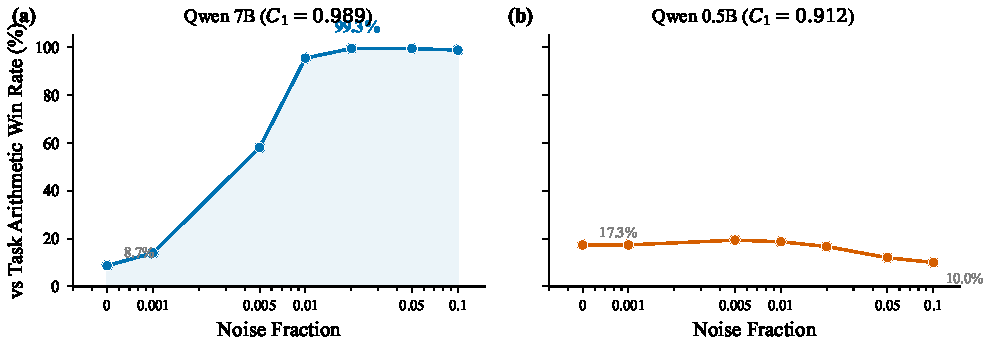
\includegraphics[width=0.85\columnwidth]{fig_c1_dissociation.pdf}
\caption{C1-gated stochastic resonance dissociation. \textbf{Left:} Qwen~7B (collinearity 0.973, C1 met)---noise produces a dramatic inverted-U, lifting composition from 8.7\% to 99.3\% vs.\ task arithmetic (+90.7 points). \textbf{Right:} Qwen~0.5B (collinearity 0.906, C1 not met)---noise produces no meaningful benefit (+2.0 points at best) and degrades monotonically. The dissociation confirms that condition C1 (suboptimality) gates the stochastic resonance effect, ruling out regularization (falsification condition F4).}
\label{fig:c1_dissociation}
\end{figure}

\subsection{Jazz Improvisation: Creative Emergence Through Lossy Real-Time Communication}

\emph{Note: This instance is illustrative, not validating. It provides a vivid demonstration of the framework's mechanism under divergent selection, but the evidence is documentary and anecdotal, not quantitative. It should be read as a worked example that makes the formal structure concrete, not as empirical confirmation of Theorem~1.}

\medskip
The preceding instances demonstrate convergent pathology (Sections~4.2--4.4) and computational diagnostics (Section~4.5). The dual-valence claim requires a positive instance: a case where the lossy channel mechanism produces genuine creative novelty under divergent selection.

\subsubsection{The Instance}

In ensemble jazz improvisation, each musician transmits musical intent through an inherently lossy channel: the acoustic signal, filtered by the listener's auditory processing, harmonic vocabulary, rhythmic frame, and stylistic training. No musician can perfectly decode another's intent. The residual---the gap between the player's intent and the listener's perception---is filled by the listening musician's own priors.

This is the Crawford--Sobel channel operating in real time. The ``bias'' is not strategic misalignment but \emph{ontological} misalignment: each musician has a different compression scheme (harmonic vocabulary, rhythmic frame) that partitions the continuous acoustic signal into different categories. The partition theorem applies directly: the more divergent the musical backgrounds, the coarser the mutual partitions, the larger the generative residual.

\subsubsection{The Evidence}

The mechanism is visible at the individual interaction level in documented cases:

\textbf{Miles Davis's Second Great Quintet (1964--68).} Davis deliberately assembled musicians with incompatible approaches: Herbie Hancock's bop-based harmonic vocabulary, Wayne Shorter's modal and through-composed orientation, Tony Williams's polyrhythmic extensions of Elvin Jones's approach, Ron Carter's walking bass tradition. Davis gave minimal direction---often just a sketch, sometimes only a tempo and a key center. The lossy channel between musicians was maximally wide. The result---documented on records including \emph{E.S.P.}, \emph{Miles Smiles}, \emph{Nefertiti}, and \emph{Filles de Kilimanjaro}---was the most consequential period of harmonic innovation in post-bop jazz. Forms dissolved. Preset harmonic schemes gave way to what the musicians called ``time, no changes''---structures that emerged from interaction rather than from composition.

The key observation: the innovations were not composed by Davis and executed by the band. They were \emph{emergent from the lossy channel}. Hancock has described moments where he played what he thought was a ``wrong'' chord---a misinterpretation of the harmonic trajectory Davis intended---and Davis responded not by correcting him but by incorporating the chord into a new direction. The ``error'' at level~$N$ (fidelity to the intended harmonic progression) became information at level~$N{+}1$ (a new harmonic pathway that neither musician would have composed alone). This is Atlan level-crossing in real time.

\textbf{Ornette Coleman's ``harmolodics'' (1958--).} Coleman's \emph{Free Jazz} (1960)---two simultaneously improvising quartets with no predetermined harmony---represents the extreme case: the lossy channel is maximally wide, the compression is extreme, and the selection is purely divergent. The result was a genuine artistic revolution---not noise, not chaos, but structured novelty arising from forced reconstruction across incompatible frames.

\textbf{Keith Jarrett's solo concerts (1973--).} Jarrett's \emph{The K\"{o}ln Concert} (1975) demonstrates the mechanism operating within a single musician. Playing entirely improvised material on an unfamiliar, partially broken piano, Jarrett was forced to reconstruct his musical intent through an instrument that resisted his habitual patterns. The lossy channel was physical---the piano's mechanical limitations compressed his intentions---and the reconstruction drew on his gospel, classical, and jazz training simultaneously. The result was not what he would have composed on a functioning Steinway. It was something neither he nor the piano ``contained.''

\subsubsection{The Condition Check}

\begin{center}
\begin{tabular}{@{}cp{10cm}@{}}
\toprule
\textbf{Cond.} & \textbf{Status in Jazz Improvisation} \\
\midrule
C1 & \textbf{Met.} Collective output of musicians playing from a score is bounded by the composition. Improvisation has room for improvement. \\
C2 & \textbf{Met.} Musical cognition is nonlinear: a note within the expected harmonic frame produces a qualitatively different response than one outside it. \\
C3 & \textbf{Met.} Harmonic reinterpretations can reach the improvement region---producing new progressions that are musically valid. \\
C4 & \textbf{Met.} The jazz aesthetic values collective innovation ($N{+}1$) over individual fidelity to a score ($N$). \\
C5 & \textbf{Met.} Skilled jazz musicians degrade gracefully under misinterpretation. Training provides the redundancy that allows productive absorption of noise. \\
\bottomrule
\end{tabular}
\end{center}

\subsubsection{What This Validates}

This instance completes the dual-valence evidence base. The Dysmemic Pressure instance (Section~4.2) demonstrates the identical mechanism under convergent selection. Jazz improvisation demonstrates the mechanism under divergent selection. Same channel structure. Same compression. Same forced reconstruction. Different selection criterion. Different valence.

The jazz instance also demonstrates why Corollary~\ref{cor:brittleness} (the Brittleness Trap) matters in creative domains. A musician who cannot absorb misinterpretation without losing function---a brittle player---cannot participate in generative improvisation. Training provides the redundancy (C5) that allows noise to become signal.


\subsection{Hierarchical Context Distillation: Functional Compression}

This final instance addresses a completeness question: if compression inevitably produces problems or novelty, how do functional hierarchies exist at all? Three formalisms---cognitive limits \citep{miller1956,sweller1988}, the Information Bottleneck principle \citep{tishby1999}, and Ashby's Law of Requisite Variety---converge on the answer: middle management performs information compression that is \emph{necessary for scale}, not pathological. The manager's formal job is the IB objective: minimize $I(X; T)$ while maximizing $I(T; Y)$. Mission command---transmit intent, not instruction; authorize deviation when local conditions require it---is hierarchical distillation under divergent selection. The valence is \textbf{design-dependent}: well-calibrated compression is functional; mis-calibrated compression is the Context Trap. This instance contributes no new empirical data but integrates established results to show that the framework's predictions about functional lossy channels are consistent with the organizational design literature.


\subsection{Cross-Instance Synthesis}

\begin{center}
\begin{tabular}{@{}lllll@{}}
\toprule
\textbf{Instance} & \textbf{Substrate} & \textbf{Channel} & \textbf{Selection} & \textbf{Valence} \\
\midrule
Dysmemic Pressure & Org.\ hierarchy & Pref.\ divergence & Internal fitness & Conv.\ $\to$ Cage \\
Variance Compression & Strategic language & Legal formalization & Defensibility & Conv.\ $\to$ ling.\ cage \\
Structural Immunity & Legal architecture & Arbitration + conf. & Repeat-player & Conv.\ $\to$ suppression \\
Activation Space & Comp.\ geometry & High-dim.\ projection & Composition quality & Div.\ $\to$ diagnostic \\
Jazz Improvisation & Musical interaction & Acoustic/cognitive & Aesthetic novelty & Div.\ $\to$ emergence \\
Hier.\ Distillation & Cognitive arch. & Capacity limits & Relevance pres. & Both $\to$ design-dep. \\
\bottomrule
\end{tabular}
\end{center}

No two instances share a substrate. The formal structure is identical across all six. The two instances with quantitative condition verification (Variance Compression and Activation Space) demonstrate that the five conditions are not merely qualitatively plausible but measurably present in real data. The four supporting instances provide breadth: three convergent-pathology cases, one creative emergence case, and one functional-compression case. The dual-valence claim---that the same mechanism produces dysfunction under convergent selection and creativity under divergent selection---is supported by instances on both sides of the valence divide, with the Dysmemic Pressure (convergent) and Jazz Improvisation (divergent) instances sharing identical channel structure under opposite selection criteria.


% ============================================================
% SECTION 5: LIMITATIONS, FALSIFICATION, AND OPEN QUESTIONS
% ============================================================
\section{Limitations, Falsification, and Open Questions}

\subsection{What the Theory Claims and Does Not Claim}

The framework claims that five conditions are jointly \emph{sufficient} for net-beneficial noise in a two-level system. It does not claim they are necessary. It does not claim that noise is generally good. It does not claim that the same optimal noise level applies across substrates. It claims: check these five conditions; if all hold, moderate noise helps; if any fails, no guarantee.

The framework also claims that the same lossy-channel mechanism produces both organizational dysfunction and creative emergence, with the valence determined by the selection environment. It does not claim that dysfunction and creativity are identical---it claims they share a root cause.


\subsection{Falsification Conditions}

\textbf{F1: Counterexample to sufficiency.} All five conditions verified as met, and the inverted-U does not appear. Zero counterexamples found across 500 Monte Carlo configurations and six mechanisms.

\textbf{F2: Mechanism-independent benefit.} Noise produces benefit with zero conditions met. Not observed.

\textbf{F3: Symmetric valence.} Two systems with identical channel properties but different selection criteria produce the same output valence. Would invalidate Proposition~\ref{prop:dualvalence}.

\textbf{F4: Scale-independent SR.} The companion activation space experiment: noise helps equally at 7B (C1 met) and 0.5B (C1 not met). Would reduce the mechanism to regularization. \emph{Ruled out}: noise produces +90.7 points at 7B vs.\ +2.0 points at 0.5B (Section~4.5).

\textbf{F5: Beneficial noise in a linear system.} Noise produces net system benefit where the integration function is strictly linear and the Jensen gap is identically zero. Not observed in computational null model.


\subsection{Limitations of the Computational Validation}

\textbf{Sufficient vs.\ necessary.} The 8.9\% of configurations showing benefit despite condition violations means the conditions define a conservative boundary. Tightening the gap between sufficient and necessary is open.

\textbf{Ensemble C4 test failure.} The C4 violation test for ensemble diversity did not effectively induce violation because the hard XOR problem makes all individual predictors weak regardless of weighting. The theory's prediction is correct; the test failed to create the intended condition.

\textbf{C2 steepness threshold.} The minimum steepness required for a meaningful Jensen gap is identified (between sigmoid and polynomial) but not quantified. Connection to \citet{chapeau1997} on generalized SR for arbitrary nonlinearities.

\textbf{Crawford--Sobel simplifications.} The one-sender-one-receiver model with uniform priors. Real hierarchies involve multiple senders, heterogeneous priors, and reputation effects.


\subsection{Open Questions}

\textbf{O1: Multi-level cascades.} The theorem covers two levels. Does it compose across $N$ levels? Connection to \citet{rosas2024} on hierarchical emergence via computational mechanics.

\textbf{O2: Dynamic environments.} Static conditions assumed. In non-stationary environments, the optimal noise level must track shifting thresholds.

\textbf{O3: Quantitative $\sigma^*$ prediction.} The theorem guarantees existence but not a closed-form. The empirical calibration approach ($\sigma = k \cdot f(\text{operating point})$) is currently the most defensible prescription.

\textbf{O4: Connection to causal emergence.} \citet{hoel2013} proved effective information can peak at the macro level. The relationship between our Theorem~1 and positive causal emergence is suggestive but unproved.

\textbf{O5: Tightening C4.} The integral condition is correct but hard to verify a priori. A simpler sufficient condition on $\beta/\alpha$ and $L$ that implies the integral condition would be practically valuable.

\textbf{O6: Additional mechanism classes.} Theorems~\ref{thm:1a}, \ref{thm:1b}, and \ref{thm:1c} establish three proof paths to the inverted-U under the shared conditions. Whether additional mechanism classes exist---beyond threshold SR, Jensen gap, and opposing monotones---is an open empirical question.


\subsection{What a Null Result Means}

The framework makes precise predictions. Some will fail. When they do, the failure is informative:
\begin{itemize}
    \item If the activation space SR experiment fails at high collinearity, the 7B degradation is geometric collapse, not threshold failure---redirecting the engineering effort toward nonlinear decomposition. \emph{Update}: The experiment succeeded; the 7B degradation is threshold failure amenable to noise-assisted recovery (+90.7 points at $\sigma^* = 0.020$).
    \item If the inverted-U fails where conditions appear met, the most likely explanation is misassessed C2 or C4---the failure is diagnosable.
    \item If noise helps at 0.5B (C1 not met), the mechanism is regularization---the theory loses one instance, not its structure. \emph{Update}: Noise does not meaningfully help at 0.5B (+2.0 points, within noise), confirming the C1-gated mechanism.
\end{itemize}

The framework is designed to be wrong precisely. A theory that cannot be wrong cannot be useful.


% ============================================================
% REFERENCES
% ============================================================
\bibliographystyle{apalike}

\begin{thebibliography}{99}

\bibitem[Ashby(1956)]{ashby1956}
Ashby, W.~R. (1956).
\newblock \emph{An Introduction to Cybernetics}.
\newblock Chapman \& Hall.

\bibitem[Atlan(1979)]{atlan1979}
Atlan, H. (1979).
\newblock \emph{Entre le cristal et la fum\'{e}e}.
\newblock \'{E}ditions du Seuil.

\bibitem[Bjork and Bjork(1992)]{bjork1992}
Bjork, R.~A., \& Bjork, E.~L. (1992).
\newblock A new theory of disuse and an old theory of stimulus fluctuation.
\newblock In A.~Healy et~al. (Eds.), \emph{From Learning Processes to Cognitive Processes: Essays in Honor of William K. Estes} (Vol.~2, pp.~35--67). Erlbaum.

\bibitem[Bjork and Bjork(2011)]{bjork2011}
Bjork, R.~A., \& Bjork, E.~L. (2011).
\newblock Making things hard on yourself, but in a good way: Creating desirable difficulties to enhance learning.
\newblock \emph{Psychology and the Real World}, 56--64.

\bibitem[Blau and Michaeli(2018)]{blau2018}
Blau, Y., \& Michaeli, T. (2018).
\newblock The perception-distortion tradeoff.
\newblock \emph{CVPR 2018}.

\bibitem[Blau and Michaeli(2019)]{blau2019}
Blau, Y., \& Michaeli, T. (2019).
\newblock Rethinking lossy compression: The rate-distortion-perception tradeoff.
\newblock \emph{ICML 2019}.

\bibitem[Chapeau-Blondeau(1997)]{chapeau1997}
Chapeau-Blondeau, F. (1997).
\newblock Stochastic resonance in the Heaviside nonlinearity with white noise and arbitrary signal.
\newblock \emph{Physical Review E}, 55(2), 2016.

\bibitem[Crawford and Sobel(1982)]{crawford1982}
Crawford, V.~P., \& Sobel, J. (1982).
\newblock Strategic information transmission.
\newblock \emph{Econometrica}, 50(6), 1431--1451.

\bibitem[Edmondson(1999)]{edmondson1999}
Edmondson, A. (1999).
\newblock Psychological safety and learning behavior in work teams.
\newblock \emph{Administrative Science Quarterly}, 44(2), 350--383.

\bibitem[Gammaitoni et~al.(1998)]{gammaitoni1998}
Gammaitoni, L., H\"{a}nggi, P., Jung, P., \& Marchesoni, F. (1998).
\newblock Stochastic resonance.
\newblock \emph{Reviews of Modern Physics}, 70(1), 223.

\bibitem[Hargadon and Sutton(1997)]{hargadon1997}
Hargadon, A., \& Sutton, R.~I. (1997).
\newblock Technology brokering and innovation in a product development firm.
\newblock \emph{Administrative Science Quarterly}, 42(4), 716--749.

\bibitem[Hoel et~al.(2013)]{hoel2013}
Hoel, E.~P., Albantakis, L., \& Tononi, G. (2013).
\newblock Quantifying causal emergence shows that macro can beat micro.
\newblock \emph{Proceedings of the National Academy of Sciences}, 110(49), 19790--19795.

\bibitem[Janis(1972)]{janis1972}
Janis, I.~L. (1972).
\newblock \emph{Victims of Groupthink}.
\newblock Houghton Mifflin.

\bibitem[Kirkpatrick et~al.(1983)]{kirkpatrick1983}
Kirkpatrick, S., Gelatt, C.~D., \& Vecchi, M.~P. (1983).
\newblock Optimization by simulated annealing.
\newblock \emph{Science}, 220(4598), 671--680.

\bibitem[Kosko and Mitaim(2003)]{kosko2003}
Kosko, B., \& Mitaim, S. (2003).
\newblock Stochastic resonance in noisy threshold neurons.
\newblock \emph{Neural Networks}, 16(5--6), 755--761.

\bibitem[Krogh and Vedelsby(1994)]{krogh1994}
Krogh, A., \& Vedelsby, J. (1994).
\newblock Neural network ensembles, cross validation, and active learning.
\newblock \emph{NIPS 1994}.

\bibitem[McDonnell and Abbott(2009)]{mcdonnell2009}
McDonnell, M.~D., \& Abbott, D. (2009).
\newblock What is stochastic resonance? Definitions, misconceptions, debates, and its relevance to biology.
\newblock \emph{PLoS Computational Biology}, 5(5), e1000348.

\bibitem[McEntire(2026)]{mcentire2026structural}
McEntire, J. (2026).
\newblock The Shape of the Problem: Domain-Invariant Structural Signatures in Activation Space Enable Cross-Domain Solution Transfer.
\newblock \emph{arXiv preprint}, 2026.

\bibitem[Miller(1956)]{miller1956}
Miller, G.~A. (1956).
\newblock The magical number seven, plus or minus two.
\newblock \emph{Psychological Review}, 63(2), 81--97.

\bibitem[Pavlik and Anderson(2005)]{pavlik2005}
Pavlik, P.~I., \& Anderson, J.~R. (2005).
\newblock Practice and forgetting effects on vocabulary memory: An activation-based model of the spacing effect.
\newblock \emph{Cognitive Science}, 29(4), 559--586.

\bibitem[Pyc and Rawson(2009)]{pyc2009}
Pyc, M.~A., \& Rawson, K.~A. (2009).
\newblock Testing the retrieval effort hypothesis: Does greater difficulty correctly recalling information lead to higher levels of memory?
\newblock \emph{Journal of Memory and Language}, 60(4), 437--447.

\bibitem[Rosas et~al.(2024)]{rosas2024}
Rosas, F.~E., Mediano, P.~A.~M., Jensen, H.~J., Seth, A.~K., Barrett, A.~B., Carhart-Harris, R.~L., \& Bor, D. (2024).
\newblock Reconciling emergences: An information-theoretic approach to identify causal emergence in multivariate data.
\newblock \emph{PLoS Computational Biology}.

\bibitem[Sutton and Barto(2018)]{sutton2018}
Sutton, R.~S., \& Barto, A.~G. (2018).
\newblock \emph{Reinforcement Learning: An Introduction} (2nd ed.).
\newblock MIT Press.

\bibitem[Sweller(1988)]{sweller1988}
Sweller, J. (1988).
\newblock Cognitive load during problem solving: Effects on learning.
\newblock \emph{Cognitive Science}, 12(2), 257--285.

\bibitem[Tishby et~al.(1999)]{tishby1999}
Tishby, N., Pereira, F.~C., \& Bialek, W. (1999).
\newblock The information bottleneck method.
\newblock \emph{Proceedings of the 37th Allerton Conference}.

\bibitem[Vaughan(1996)]{vaughan1996}
Vaughan, D. (1996).
\newblock \emph{The Challenger Launch Decision}.
\newblock University of Chicago Press.

\bibitem[von Foerster(1960)]{vonfoerster1960}
von Foerster, H. (1960).
\newblock On self-organizing systems and their environments.
\newblock In \emph{Self-Organizing Systems} (pp.~31--50). Pergamon.

\bibitem[Vuori and Huy(2016)]{vuori2016}
Vuori, T.~O., \& Huy, Q.~N. (2016).
\newblock Distributed attention and shared emotions in the innovation process: How Nokia lost the smartphone battle.
\newblock \emph{Administrative Science Quarterly}, 61(1), 9--51.

\bibitem[Weick(1979)]{weick1979}
Weick, K.~E. (1979).
\newblock \emph{The Social Psychology of Organizing} (2nd ed.).
\newblock McGraw-Hill.

\bibitem[Wilson et~al.(2019)]{wilson2019}
Wilson, R.~C., Shenhav, A., Straccia, M., \& Cohen, J.~D. (2019).
\newblock The eighty five percent rule for optimal learning.
\newblock \emph{Nature Communications}, 10(1), 4646.

\end{thebibliography}

\end{document}
